% Multiple Choice Question 19 to 20 (2 questions)

% \par\noindent\rule{0.75\textwidth}{0.5pt} 
\textbf{See the instruction for questions \inteval{\value{question}+1} to \inteval{\value{question}+2}.} 

\begin{center}
    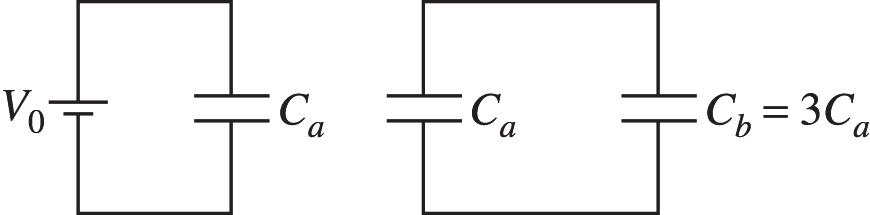
\includegraphics[scale=0.3]{images/img-009-011.png}
\end{center}

A capacitor of capacitance $C_{a}$ is first charged to a voltage $V_{0}$, as shown above on the left. Without losing any charge, the capacitor is now disconnected from the voltage source and connected to a second initially uncharged capacitor of capacitance $C_{b}$ that is three times $C_{a}$, and the circuit is allowed to reach equilibrium, as shown above on the right. 

\begin{questions}
\setcounter{question}{18}

% Multiple Choice Question 19
\question
If $Q_{a}$ is the new charge on capacitor $C_{a}$, the charge $Q_{b}$ on capacitor $C_{b}$ is given by

\begin{choices}
    \choice $0$
    \choice $Q_{a} / 3$
    \choice $Q_{a} / 2$
    \choice $Q_{a}$
    \choice $3 Q_{a}$
\end{choices}

% Multiple Choice Question 20
\question
The new voltage across capacitor $C_{a}$ is $V_{a}$. How does this new voltage compare with the original voltage of $V_{0}$?

\begin{choices}
    \choice $V_{a} >V_{0}$ 
    \choice $V_{a} <V_{0}$ 
    \choice $V_{a} =V_{0}$
    \choice It depends on the value of $C_{a}$.
    \choice It depends on the value of $C_{b}$.
\end{choices}

\end{questions}
